% Which style? IEEE is two columns, article is one column with all text.
% \documentclass{article}
\documentclass[article, 10pt]{IEEEtran}

\usepackage{subcaption}
\usepackage{verbatim}
\usepackage{svg}
\usepackage{graphicx} % Required for inserting images
\usepackage{booktabs}


%%%%%%%%%%%%%%%%%%%%%%%%%%%%%%%%%%%%%%%%%%%%%%%%%%%%%%%%%%%%%%%%%%%%%%%%%%%%%%%%%%%%%%%%%%%%%%%%
%%%%%%%%%%%%%%%%%%%%%%%%%%%%%%%%%%%%%%%%%%%%%%%%%%%%%%%%%%%%%%%%%%%%%%%%%%%%%%%%%%%%%%%%%%%%%%%%
\begin{document}


\title{Efficacy of World Models in Tackling Bomberman}
\author{Alois Bachmann, Colin Fyock, Caius Mihai Hetko \\
Heidelberg University, Germany
\date{September 2026}
}

\maketitle

%%%%%%%%% ABSTRACT
\section{Abstract (Colin)}\label{sec:0_abstract}
In this paper, we compare the performance of Q-learning models that utilize world models for training and planning on the task of winning and scoring points in Bomberman. We built several agents for this task with varying world models, and one without. Our second best performing model is DynaQ, a tabular Dyna-Q whose world model replays previously observed transitions for background planning. The best performing model was QWM, a deep Q-learning agent with a learned World model built on existing architecture\cite{dong2026qwm}. QWM uses its learned world model for decision-time planning through a tree search. Using an average of 1000 rounds against rule based agents as a benchmark for evaluating our models, QWM achieved an average score/round of 3.87, survived 63\% of the rounds and with only 242 suicides. Comparatively, DynaQ achieved a mean score of 3.71, survived 49.8\% of the rounds, but had 408 suicides. The closeness in score of the models required further testing against each other. The mean scores continued to not be statistically significant, but the QWM agent showed a clear in survival and a low number of suicides. We conclude that the architecture of QWM is an apt architecture for the given problem of gaining points and winning at Bomberman, though its advantage lies in survival, and comes at the cost of a much longer inference time.
% Swap out metrics for real numbers when we decided what exactly we are comparing the agents against each other on
% From the stats it looks like we should be saying that neither is strictly better performing, but QWM has a slight performance lead over DynaQ, though as the p-value shows from the table it is not significant. Need to edit the abstract to reflect whichever we decide on in the results section.

%%%%%%%%% BODY TEXT
% Briefly state the problem you are trying to solve and explain why the task is worthwhile and challenging.
\section{Introduction (Colin)}\label{sec:1_introduction}
Reinforcement learning for games is an interesting application of artificial intelligence, and has gained significant attention in recent years. The process of using RL algorithms to solve games acts as a good example of the ability for machines to learn and generalize around a specific problem set with given environment variables. A classical example of applying reinforcement learning to games is building machines that can perform well in the board games Chess and Go. Both games involve no randomness, and are purely built on moves and actions of the players in them. This makes them good test-cases for RL as the board is only affected by their actions, and those actions affect the future states. The rewards that can be encoded into the RL agents also naturally follow in these games, as actions like taking enemy pieces or promoting a pawn to a more powerful piece in Chess act as positive rewards. Losing pieces, getting placed in check, or losing the game could count as negative rewards. Other more abstract rewards like optimal moves and positioning could be encoded as additional information for the algorithm to work off of.

Bomberman is its own challenging problem to solve, and is complex in different ways compared to Chess or Go. Firstly, Bomberman is a four-player game, which means there is more than one opponent to adapt strategy to. Each of these four players makes a move each time slice simultaneously. Secondly, Bomberman adds an aspect of randomness. Based on the random seed, the layout of boxes, coins within those boxes, and the starting corner of each agent is randomly selected. This makes it so there is no certainty of coins being in certain places, and incentivizes agents to develop a skill for searching for, collecting, or bombing crates for coins. Similar to Chess and Go, Bomberman has strong delayed rewards and consequences. Agents choosing to bomb crates to reveal coins or defeat enemies only pays off after the bomb sits and ticks down, exploding four time steps later. In between placing the bomb and it exploding, the agent must navigate out of its own blast or be killed. Even after that, if a bomb destroyed a crate and revealed a coin, the agent then has to navigate around boxes and enemy bombs in order to turn that original bomb into the measurable reward of collecting a coin. The agent has to learn from its interaction with the environment on how to deal with the delayed consequences of placing a bomb. Bomberman also has expensive and irreversible mistakes the agent can make, like bombing itself. Despite one agent dying not immediately ending the game, dying means that the agent has less opportunity to acquire coins or bomb enemies in later states, thereby decreasing its theoretical future yield of points. Each of these problems add up to Bomberman being a challenging problem for RL to adapt to. Though Bomberman can be effectively played with several techniques, our paper solely focuses on reinforcement learning approaches. 

In this report, we will provide an overview of the agents we created to optimally play Bomberman, explain their algorithms and training and ultimately evaluate their performance against the provided rule-based agents, and against our own models. We will discuss their unique advantages and disadvantages when it comes to attempting to be the best agent in Bomberman.


% Testing models on games is a fascinating example of the power of Artificial Intelligence and Reinforcement Learning's ability to adapt to problems bound by specific environmental rules. Utilizing RL to play video games has existed as testbed for RL for decades\cite{relevant citation}. Existing literature mostly covers games where only two players compete against each other to achieve victory. Bomberman is a deviation from this scheme as it employs four players on the board instead of two. Bomberman is additionally challenging because of its delayed rewards and punishing lose state. Agents choosing to bomb crates to reveal coins or defeat enemies only pays off after the bomb sits and ticks down, exploding three time steps later. Despite dying not ending the game immediately in Bomberman, dying means that the agent has less opportunity to acquire coins or bomb enemies in later states, thereby decreasing its theoretical future yield of points.


% Outline:
% - Playing games has been a standard test of RL algorithms in history 
% - Utilizing a world model to make decision-time search has a history, and leads into the architecture that we used. World model dreaming paper if we talk about world\_model\_agent?
% - We are doing these but applying it to a game with more enemies than the traditional Chess or Go offers, leading to a complicated and interesting problem to try and solve


% Describe the task in more detail and give an overview of possible solution methods (here: different approaches to reinforcement learning that you considered).
\section{Background}\label{sec:2_background}
% Background here. Baseline of x.

% Could have an interesting subsection here talking about devised strategies that are tournament specific, like an agent that collects a few coins then kills itself as to not let any other agents win.
\subsection{Bomberman Strategies}
Bomberman is a game that can be played utilizing several different strategies and the way we built our agents reflects the goals and sub-goals we expect our agent to aim towards on its way to victory. 

\subsection{Q-Learning}

\textit{Primary author: Caius Mihai Hetko.}

Q-learning estimates the expected return of taking action $a$ in state $s$ and then following the learned policy. For an observed transition $(s,a,r,s')$, the selected entry is updated according to
\begin{equation}
Q(s,a) \leftarrow Q(s,a) + \alpha \left[r + \gamma \max_{a' \in \mathcal{A}(s')} Q(s',a') - Q(s,a)\right],
\end{equation}
where $\alpha$ is the learning rate and $\gamma$ discounts future rewards. This formulation is suitable for Bomberman because its action space is discrete, but a purely model-free agent uses a transition only when it is observed. That is inefficient for events such as bomb explosions, coin collection, and deaths, whose causes and rewards may be separated by several steps.

Dyna-Q combines direct Q-learning with a learned model of previously observed transitions \cite{sutton1990integrated}. After updating from a real transition, the agent samples transitions from the model and applies additional Q-learning updates as background planning. The method therefore reuses experience without requiring the agent to recreate the same situation in the environment. It also provides a computationally inexpensive contrast to QWM: DynaQ plans during training by replaying stored outcomes, whereas QWM uses a learned latent model for search while selecting actions.

\subsection{World Models}

The world model consists of a student encoder, a teacher encoder, and an action-conditioned prediction network. Given the observation at time step \(t\), the student encoder produces a latent state representation \(z_t\). The teacher encoder produces a target representation \(\bar{z}_{t+1}\) for the observation at the subsequent time step. The prediction network receives \(z_t\) together with the executed action \(a_t\) and predicts the latent representation of the next state:
\[
\hat{z}_{t+1} = f_{\theta}(z_t, a_t).
\]
Training minimizes the discrepancy between the predicted representation \(\hat{z}_{t+1}\) and the teacher representation \(\bar{z}_{t+1}\). The teacher parameters are updated as an exponential moving average (EMA) of the student parameters. This prevents the prediction target from changing too abruptly and avoids directly optimizing the network to reconstruct raw observations.


% Describe how you organized the team work, planned your time to meet the deadline, distributed subtasks among the team members, and collaborated to produce the best possible results. If you use deep learning, also describe where and how you allocated the required hardware ressources for training (e.g. Google Colab)
\section{Project Planning (Colin)}\label{sec:3_projectplanning}
Our organization of team work was broken down into research, testing, agent building, and finishing touches. We organized team work through a discord group chat and a GitHub where we stored all of the code and agents we were working on together. The discord group chat was used to schedule calls and discuss the material as was needed, and towards the end of the project we moved to having daily calls to make sure we met every deadline. We organized team work differently depending on the phase of the project we were on. 

During the first phase, we researched different architecture in reinforcement learning to pick out which would give us the best shot of winning the tournament. The research included reading through the existing literature on models like DreamerV3\cite{hafner2023dreamerv3}, JEPA\cite{assran2023ijepa}, and several papers on world models\cite{dong2026qwm}\cite{ha2018worldmodels}\cite{schrittwieser2020mastering}. World models and DreamerV3 looked the most promising from the beginning. Our second phase was splitting up and doing early testing on what we though was promising or would be interesting experiments. Colin did early testing with a basic TD Q-learning agent called basic agent resulted in little success on any scenario more complicated than coin heaven. Alois did tests with the Dreamer architecture, but it performed poorly and failed to materialize any good results. A paper on genetic algorithms, and another on hierarchy planning both looked good, but through trying each they performed poorly in Bomberman. We concluded that utilizing world models was the most promising architecture for Bomberman. We found that world models could be used in two different ways, for training and for planning. Caius developed an early tabular Q-learning model that used a basic world model to feed in additional recorded transitions into the training regiment. This model acted as a base for developing the further models, and eventually the two best agents: DynaQ and QWM. In our agent building phase we developed the DynaQ model as a combination of the best parts and reward shaping of the basic agent and the world model of the tabular Q-learning. DynaQ's world model was primarily used for training. The QWM agent went further by utilizing a world model for planning and training, along with deep learning. The training of both of these agents happened partially in parallel to have two results for the submission. We budgeted time for the end of the project period to further test and train the QWM and DynaQ agents against each other. We then used the rule based agent as a benchmark to evaluate if training against each other generalized to fighting the rule based agents. Each agent or test we ran acted as a stepping stone for the agents that would come in the future.

The final phase involved running final tests, evaluating our models against one another, and splitting up paper writing. The final tests we ran were to compare our agents in various scenarios and in direct combat against on another, and build metrics on that to determine which we should submit to the tournament. These results are shown in Tables~\ref{DynaQ and QWM Comparison on Four Tasks}, ~\ref{tab:DynaQ vs QWM Comparison tournament/duel}, and~\ref{tab:Primary and Efficiency Metrics per task for DynaQ and QWM}. The results of the head-to-head test showed that the QWM agent beat out the DynaQ agent in rounds won, win rate, survival rate, mean score, coins per round, kills per round, all with significantly less suicides. We then transitioned to paper writing. To make writing the simplest we assigned sections which each person would oversee, but not necessarily write in full. Most sections in the report include the voices of all our team members, especially portions of training and evaluation as we used different hardware and trained at different times. The sections of the paper were split as following: Colin oversees Introduction and Project Planning, Alois oversees Training and Methods, and Caius oversees Background and Conclusion. Experiments and results had no lead as we wrote that section in equal parts and had at least once part in that section written by each person similar to the training section.
% Do we want to touch on future work?

The QWM agent utilized deep learning, which was trained locally on Alois' computer. This computer has a [GPU AND CPU, ADDITIONAL PARTS?]. Alois also utilized an activation function that was written prior to the project's start date. This activation function...
% ^ Alois needs to complete this paragraph ^

% Firstly, we broke into different sections researching various paths of reinforcement learning we could utilize in our agent architecture to effectively play Bomberman. We split the research between the three of us and looked for existing papers on world models and examples of reinforcement learning performing well in games.

% We knew early on that we wanted to focus on using world models to try to play Bomberman. 

% Project planning here. Bring up the models that we developed on the way to getting to the dynaQ and QWM agents, since we are not mentioning them in the abstract/introduction. Talk about them like a stepping stone on developing the models that we are submitting and running metrics against as our best models.


% Describe how you specialized the general methods from the "background" section for the concrete task. Explain and justify crucial design choices, list the variants to be tested in the experiments, and design a methodology for systematic testing of agent performance (e.g. define performance metrics). You may also describe approaches you tried and abandoned later, including the reasons. Include references to relevant literature. Recall that each team should implement at least two different agents.
\section{Methods}\label{sec:4_methods}
% Methods used here

\subsection{Methodology for Systematic Testing of Agent Performance}\label{sec:evaluation_methodology}
We evaluated both candidate agents with training disabled and greedy action selection. Each condition in the staged comparison contains 1,000 rounds. The same scenario definitions were used for both agents: coin navigation in \texttt{coin-heaven}, crate clearing in \texttt{loot-crate}, a classic scenario with peaceful and coin-collector opponents, and competitive play against three provided rule-based agents. Win rate denotes the share of rounds in which the evaluated agent achieved the highest score, not including tied highest scores. Survival rate denotes the share of rounds in which the agent remained alive until the round ended. We additionally report mean score, coins, destroyed crates, kills, and suicides. Task-specific efficiency metrics are steps and waiting actions per coin for navigation, and crates per bomb for crate clearing.

The provided rule-based agents serve as fixed benchmark opponents in the competitive task and during the first DynaQ training branch. They were not evaluated as a separate candidate with the same 1,000-round protocol on all four tasks. We therefore use them to measure performance against a consistent opponent. Beating the rule-based agent is a good indicator that an agent will stand a chance in the final tournament against other group's agents. As shown in Table~\ref{tab:Primary and Efficiency Metrics per task for DynaQ and QWM}, both our QWM and DynaQ agents outperform rule-based agents in competitive combat.

For direct DynaQ--QWM comparisons, both agents were evaluated on 1,000 identical random seeds, with starting positions alternated to reduce slot bias. We report the paired difference $\Delta=\mathrm{DynaQ}-\mathrm{QWM}$ and a 95\% confidence interval for the mean-score difference. A negative difference therefore favors QWM. This paired design separates architectural differences from variation in board layouts and coin placement.
% We should define them as what we compared our QWM and DynaQ agents against, also talk about rule-based agents being a baseline performance-wise.

\subsection{DyanQ Agent}\label{subsec:DynaQ Methods}\label{sec:dyna_method}

\textit{Primary author: Caius Mihai Hetko.}

DynaQ is a tabular agent with six actions: movement in four directions, waiting, and placing a bomb. Its empirical world model maps each observed state--action pair to a first-in-first-out queue containing at most 100 outcomes. An outcome stores the immediate reward, the following state, whether the transition ended the round, and the actions available in the following state. Retaining several outcomes for the same pair represents stochastic changes caused by board layouts and opponent behavior better than storing only the most recent transition. After the real Q-learning update, the agent samples state--action pairs and outcomes uniformly from this model for background-planning updates.

The full board is compressed into a 20-value symbolic state. Four one-hot values encode the first direction on a shortest traversable path to the nearest visible coin. The remaining features describe the number of crates or opponents that a bomb could hit, valid neighboring movements, the direction of the previously occupied tile, safe escape directions from an active blast, whether a useful bomb can be placed with an escape route, the direction towards a useful crate-bombing position, and whether the agent already has an active bomb. Opponents are treated as blocked tiles during escape search, because a geometrically open route is not usable while another agent occupies it. These features supply task-relevant information while leaving the preference between collecting, bombing, escaping, and waiting to the learned Q-values.

Before action selection, a mask removes mechanically illegal actions and moves onto tiles that are expected to explode before they can be occupied safely. Exploration and greedy selection are then performed only over the remaining actions. The mask prevents repeated exploration of walls, crates, occupied tiles, and immediate explosions; it does not prescribe a high-level strategy. Equal Q-values are resolved randomly, avoiding the directional bias that would otherwise arise from always selecting the first action in the action list.

The feature representation was developed incrementally, first for coin navigation and later for bombing, crate search, and escape behavior. Because a change in the feature vector also changes the meaning of every Q-table key, saved models include an explicit schema version. A table is loaded only when its schema matches the current feature definition. This forces retraining after an incompatible feature change but prevents values learned for an older representation from being assigned silently to different states.

\textit{Primary author: Colin Fyock}

% A brief paragraph that was missing from Caius' markdown file was the breakdown of schema files that I used. Schemas go from 3 to 12, with 12 being the latest schema. I unfortunately did not push every schema, so some variations of the code is missing in the current repository, so we will be comparing the schema 3 and 7 code versus the current schema 12 code since I have runs from both of those and the feature vector code for both. Caisu can move this paragraph around and put it in his Methods section as he sees fit, it probably should not be the first paragraph here but wherever works.
Each schema version has a different feature vector, making the existing trained files not backwards-compatible, more is spoken on this subject in the Section~\ref{subsec:DynaQ Training}. On reflection, we should have committed the code at every schema change and saved the small experiments and agent files even if they did not amount to much. As it stands now, the schemas that fully survived are schemas 3, 7 and 12. Schema 4 and 9 have existing code in the git history but have no models to run from them. Schemas 8, 10, and 11 have models but no remaining code. Schema 12 is the latest and best performing schema, and is the one in the evaluations against the QWM agent. The surviving models are what we will go over in our evaluation and results section cover.


\subsection{QWM-Agent (Alois)}\label{sec:qwm_agent} % We can change the location later on...

\subsubsection{Planning with World Models}
%- A JEPA-like model as world model for simulation of future states

 %   - A Teacher (teacher is EMA of student) and Student model with connected latent spaces where the first model (the student) tries to predict using a prediction layer how the representation of the teacher will look like. In this case the student representation is created from the current time-step $t$ and the teacher representation is the one from $t+1$ and based on the action   taken at time $t$ the representation at $t+1$ should be predicted. 
    
%- Pre-Training via imitation learning of many pre-calculated scenarios with the rule\_based\_agent 

%- training of actor inside the latent imagination -> instability because policy the is not grounded in the reality correctly and biases are piled up (looping results and fast suicides)

%+ Planning works by "brute forcing" using a genetic algorithm -> computationally very expensive 

%-> We need a better training + planning pipeline.

%-> luckily on the 17th of August 2026 there was a paper published adressing exactly these problems: Q-Learning with World Models


Our initial approach to planning explored whether a learned world model could improve a Bomberman agent by predicting the consequences of candidate actions before they were executed in the environment. In particular, we implemented a JEPA-inspired latent dynamics model. Rather than predicting the complete next observation at the pixel (or in this case board-state) level, the model predicts a compact latent representation of the future state. Next to this representation, we also predict the value and reward for this future state using separate heads based on a candidate action. 

As an alternative to the previously explained dyna\_agnet [SECTION PENDING], we used the world model for planning rather than as a source of synthetic training data. For this we utilized the reward and value heads to predict the return of a candidate action sequence. Candidate action sequences were generated with a genetic algorithm and evaluated by rolling them out in the learned latent dynamics model. The highest-scoring sequence determined the action executed in the real environment. 

This kind of planning was inspired by the paper on hierarchical world models \cite{zhang2026hwm}. In this paper they propose this kind of planning as an efficient way to find the best trajectory in a complex environment. In the paper this was extended with sub-goals and one main goal latent state that should be reached by the model. 

If we think about goal definitions in the bomberman environment we can set a few example goals: The first one being the simplest one that the agent is the only thing left on the board. The problem with this goal is that this goal might lie a few hundreds steps into the future. At this point the world model has probably hallucinated a lot which makes a simulated path to that goal (even with subgoals) very inaccurate. 

The second possibility would be to define local goals which are more reachable (e.g.: collecting the nearest coin). A problem that would appear is that if we tell the model to only focus on one goal the agent might collect the coin very efficiently but does not look out for bombs placed by enemies and because of that it gets blown up in the next turn. So we would have to also implement the goal of safety and maybe enemy killing and also crate destruction and also make all of that very efficiently and so on. But when we have these different goals which one should we prioritize? We would have to weigh them and give the model a positive feedback if it achieves one of these goals and a negative one if he is failing in one of the goals. In other words: We need rewards and values (what is the ability to achieve different goals soon). 

This is why we use the value and reward heads to evaluate different candidate action sequences. By using this method we assumed that a higher value and reward for a given action sequence is closer to the final goal and lower reward and value is further away from it.

Using this method we can use a trained world-model to try and find the best action sequence. We do this (as proposed in the paper LeWorldModel \cite{maes2026leworldmodelstableendtoendjointembedding}) using a genetic algorithm like procedure: We sample a certain number of random action sequences text them out, take the best few and mutate them with one another to find the best action sequence. We mutate multiple times. The mutation step is the generation, the planning depth the internal simulation horizon of the world model and the population size the amount of different action sequences sampled.

\begin{figure}[!h]
     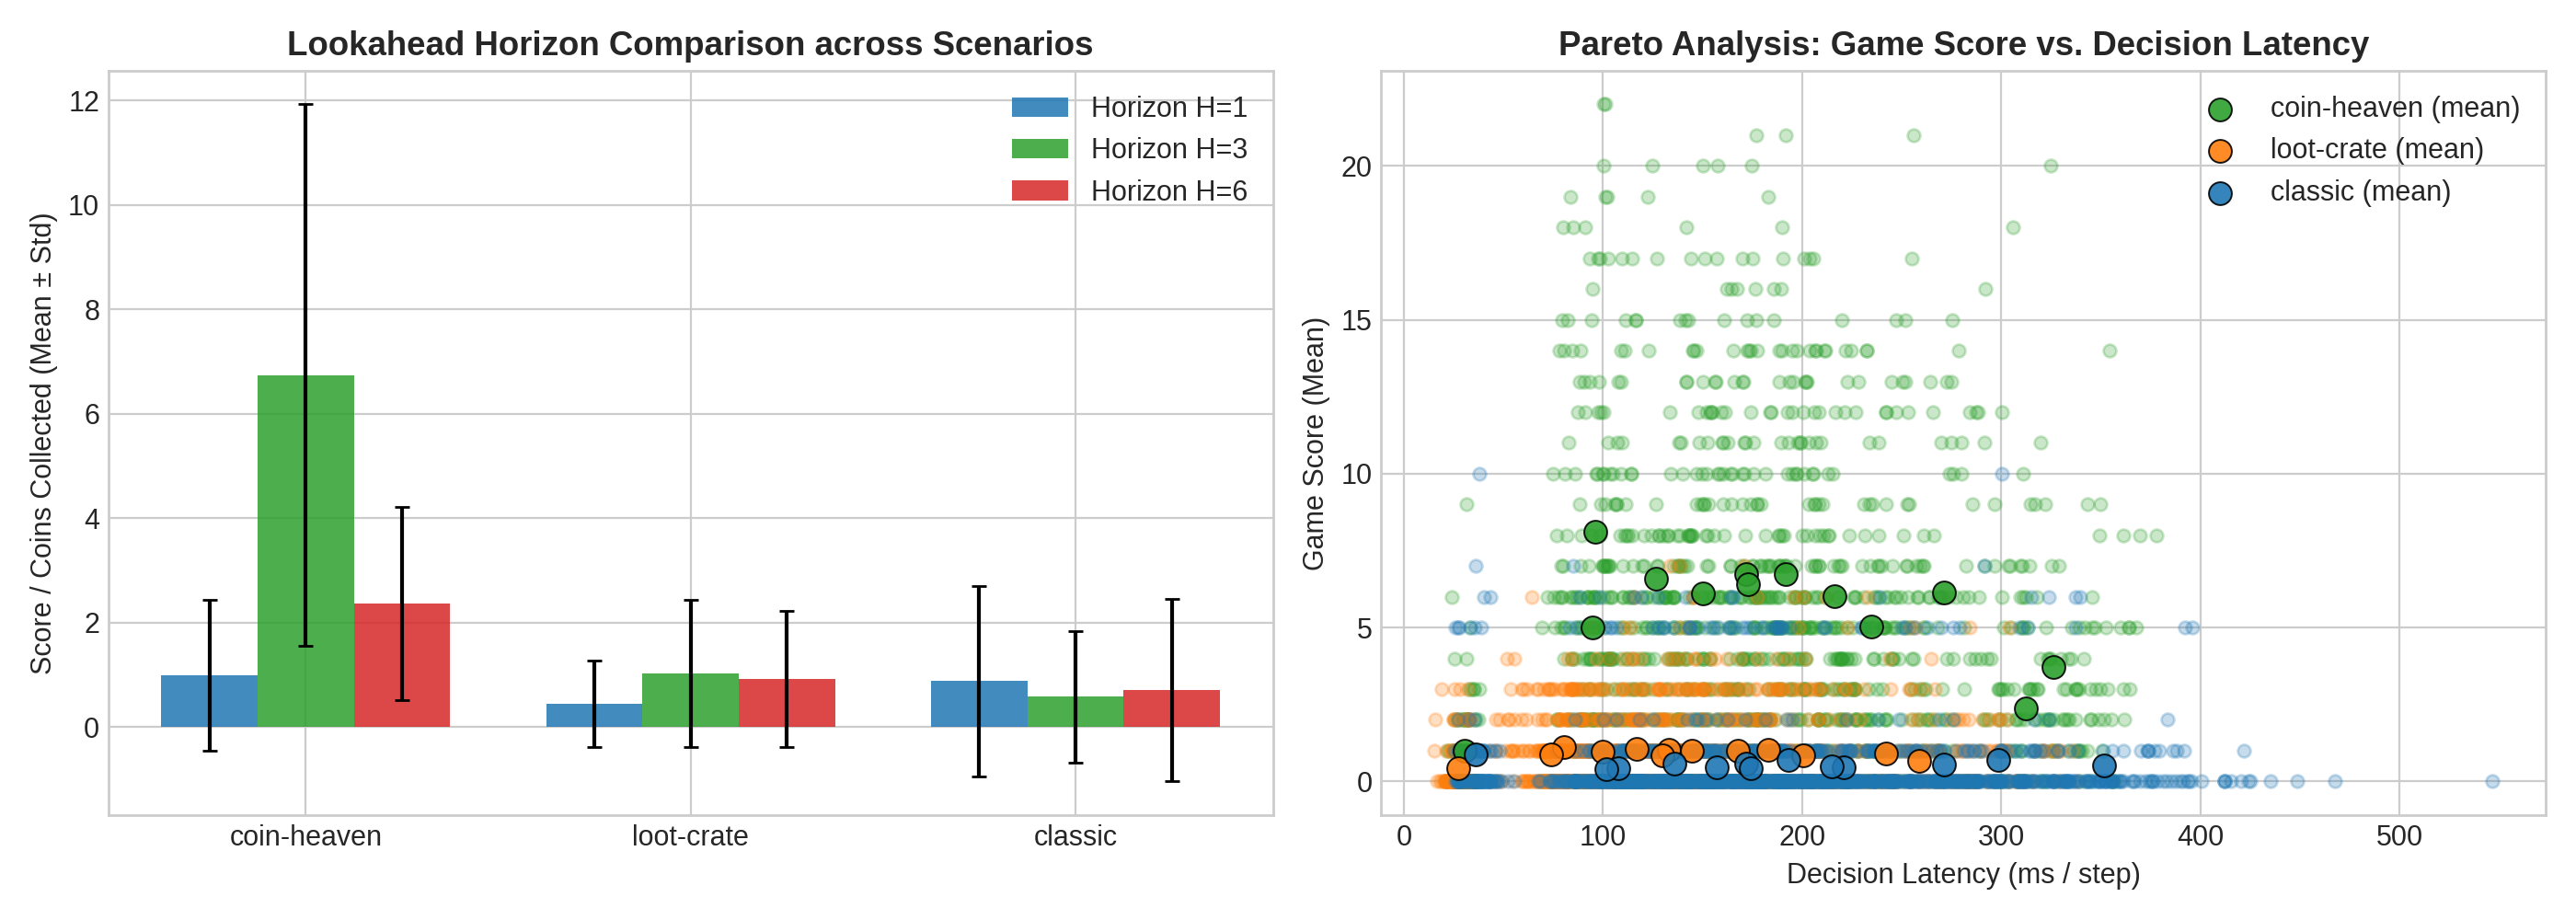
\includegraphics[width=0.96\columnwidth]{figures/ga_scenario_comparison_and_pareto.png}
     \caption{Latent planning results with pure world model with genetic algorithm and random initial action sequence sampling. Shortened environment time of max. 80 steps and no enemy agents.}
     \label{fig:pure_planning}
\end{figure}

The first thing that is visible in this plot is that we clearly have diminishing returns from long horizon planning and also long computational time. This initially seems counter-intuitive. Because we would think that if the agent can plan further into the future it would act more intelligently. 
This behavior is mainly caused by two things: 

\begin{enumerate}
    \item Not enough planning: We plainly just do not have the ability to sample enough action sequences inside our 500ms time limit to find the actual best route for a long horizon of 6 steps.
    \item Compounding world model error: Because the world model is not perfect it creates a shift in what the actual next latent representation will be every imagination step. So a small error at a low horizon can quickly compound into a very high error in longer horizons.
\end{enumerate}


Regarding the second problem: one option to improve this is that we could sample our predicted latent state using a gaussian distribution so that we do not have one deterministic state and rather a statistical one. A further improvement could be even using more binned latent representation where we decouple the information of the different bins with a new loss so that every bin only translates one information. This prevents us from mixing errors. A similar idea is used in the DreamerV3 architecture which was also tested as an option as a planning world model basis \cite{hafner2023dreamerv3}. But even with these improvements we were only able to reduce this problem and not eliminate it.

The other problem is even bigger. Because we have this hard time constraint we will only ever be able to try a set number of different action sequence and mutate them only so much. Because of this we will be stuck with sub-optimal performance. We can actually see this in figure \ref{fig:pure_planning}. We seem to be able to find reasonable action sequences for the coin-heaven but as soon as we get to the loot-crate scenario the performance degrades significantly and is not viable as a competitive agent.

This is why we need another architecture because this architecture seems to be not reasonable for the bomberman environment. (At least not with our available resources. It may be that one can achieve better results with longer and more complex training but we were not able to get this architecture to work.)

Because we primarily have to fix the planning-complexity problem we can maybe think of sampling or pruning our action sequence space more efficiently. This is why we wanted to use a policy based action sequence sampling method. The idea behind such a method would be that we train a base reinforcement learning agent which we would train in the first step to be good in the environment already and then change the architecture where we hook into an inbetween-output to use this then to predict future representations. We then would use our base agent trained without planning in the main environment to efficiently choose next actions based on our current planning step.

While we were working on this architecture we had the luck that a paper was published right on time (on the 17th of August 2026) that was also trying to make this approach work. We therefore used this paper as a basis for our further production and then also final agent \cite{dong2026qwm}.

%Before reinforcement-learning-based use of the model, we pre-trained the world model on trajectories generated by the provided rule-based agent. These trajectories contain valid state transitions and give the model examples of common Bomberman dynamics, including movement, bomb placement, explosion propagation, destruction of crates, collection of coins, and agent deaths. Imitation-based pre-training was intended to provide a useful transition model before the learned agent had collected sufficient experience on its own.

%We initially considered training the actor directly inside imagined trajectories generated by this latent world model. In principle, this would allow the agent to perform many simulated rollouts without requiring an equivalent number of environment interactions. In practice, this approach proved unstable. Small prediction errors in the learned dynamics accumulated over multi-step imagined rollouts. Consequently, the actor could exploit inaccuracies of the model instead of learning actions that are effective in the real Bomberman environment. Typical failure modes included repetitive action loops, implausible long-horizon trajectories, and policies that quickly placed themselves in lethal situations after deployment in the real environment.

%As an alternative, we used the world model for planning rather than as a source of synthetic training data. Candidate action sequences were generated with a genetic algorithm and evaluated by rolling them out in the learned latent dynamics model. The highest-scoring sequence determined the action executed in the real environment. While this approach can exploit predicted future consequences without directly optimizing a policy on simulated data, it is computationally expensive: many candidate sequences must be simulated and evaluated at every decision step. This cost is particularly problematic in Bomberman, where the branching factor is large and successful play requires reacting quickly to changing bomb timers and opponent behavior.

%These limitations motivated the transition to \emph{Q-Learning with World Models} (QWM). The QWM framework, published by Dong et al.\ on 17 August 2026, uses a learned world model for short-horizon test-time search while keeping Q-function and policy learning grounded exclusively in real environment transitions. Thus, the world model improves action selection through imagined rollouts, but model-generated trajectories are not used as training targets for the Q-function. This separation directly addresses the model-bias problem observed in our initial approach: errors in long imagined trajectories may affect a single planning decision, but they do not recursively contaminate the value-function training data. \cite{dong2026qwm}



\subsubsection{Q-Learning with World Models}

The basic idea of this agent is grounded in the paper Q-Learning with World Models \cite{dong2026qwm}. This paper describes an architecture of multiple cleverly interconnected models to achieve a policy based planning architecture. It uses one backbone agent model that learns a policy in the real environment so that it gathers a good understanding of the behaviour and physics of objects in different scenarios and take good actions based on one state. The second model is the actual world model that uses the outputs of the agents encoder model to predict the encoded state of the next time step based on some action choosen by the agent. In the original paper a big pretrained vision model was used as the vision encoder. We are not able to use such a model due to resource and time limits. Therefore we will have to train the encoder together with all the other parts of the model.

The final planning method presented in the paper is a tree search algorithm. It utilizes the ability of the model to predict q-values and rewards for every action in future time steps to efficiently prune non-promising paths to only retain a set amount of feasible paths as the final output. 

In the following we will present how we used and modified this architecture to solve the bomberman environment.



\subsubsection{Backbone model (Dueling Q-Agent)}

\begin{figure}[!h]
     \includegraphics[width=0.96\columnwidth]{figures/stage1_dqn_agent.pdf}
     \caption{Backbone DQN-Agent architecture.}
     \label{fig:dqn_agent}
\end{figure}

The first thing we train is the backbone agent on its own, without a world model and without planning. Figure~\ref{fig:dqn_agent} shows this. The idea is that if this agent is already decent at picking an action from one state, we can later use those action scores to prune the search instead of trying action sequences more or less at random, which is what we were stuck with in the genetic algorithm.

The agent is a duelling Q-agent. There is a global value head and an action specific value head. The global head says how good the state is in general, and the action head says how much better or worse one action is compared to the others in that same state. We add those together to get the action scores and then just select the highest one as the action. This is the normal duelling split. It is useful here because a lot of states in bomberman are just bad no matter what you do (you are already standing in a blast) while the difference between the six actions is still what we actually have to learn.

The encoder is two things that get fused. The first is a cnn visual encoder of the whole game state, with different channels for different informations (walls, crates, coins, bombs, agents, and so on). The second is a deterministic state extractor. This one calculates things that we do not want the cnn to have to figure out on its own, like if the agent is standing in danger and in which direction the next coin is and so on. Both of these get fused into one state. This fused state is what we call the world representation.

The world representation is then passed into the value heads. So the q-values are not computed from the raw board, they are computed from this already mixed representation. Later the world model also reads from exactly this vector.

We train this and get [here comes text needed] on the different scenarios. This is the agent without any look-ahead, so these numbers are the baseline for everything we add afterwards. We then use this as a backbone for the next step.

\subsubsection{World model}

\begin{figure}[!h]
     \includegraphics[width=\columnwidth]{figures/stage2_world_model.pdf}
     \caption{World model architecture inserted into the DQN-Agent.}
     \label{fig:world_model}
\end{figure}
\begin{figure*}[!h]
  \includegraphics[width=\textwidth]{figures/stage3_planning.pdf}
  \caption{Planning architecture utilizing the DQN-Agent and the World model.}
  \label{fig:planning}
\end{figure*}

We then train a world model to predict the next state (or in some cases states) going from one fused latent state and a selected action. Figure~\ref{fig:world_model} shows where this sits inside the DQN-Agent. The fused state and the action go into a world model trunk. The trunk predicts a world information vector, and from that vector we predict the actual things we care about with seperate heads.

These are:
\begin{enumerate}
    \item the reward gotten in that world state
    \item a value prediction of that latent world
    \item $\Delta z$, the fused state difference from the previous fused latent state to the next one
\end{enumerate}

The third one is the important design choice. If we asked the model to predict the full latent vector every time it would have to re-predict walls and coins that did not even move. With $\Delta z$ it only has to predict the changes, and the next fused state is just the old one plus that difference. This is also how we get more than one step. We add the predicted difference, treat that as the new fused state, and do the same thing again. The problem is of course that a small error in $\Delta z$ gets added again at the next step, which is the same compounding problem we already had with the earlier world model.

We also train a legal action prediction head. This head predicts which actions are legal to take in that predicted state. We use this later for prunning of invalid action sequences. We cannot just take the legal actions from the current real board and keep them for the whole rollout, because after one step a tile can be blocked, or a bomb can be ticking, or the agent might already have a bomb down. So the legal set has to be predicted together with the state.

This model is trained in different steps. In the beginning we freeze the dqn agent and really only train the world model. The dqn already produces a fused state that means something, and if we train both at the same time that state keeps moving and the world model is chasing a target that changes underneath it. We train the different heads and the world model trunk so it can accuratly predict the effects of one action on the environment. [here comes text needed]



\subsubsection{Tree-search Planning}


Using the trained world model and dqn agent we then finally go over to planning. Figure~\ref{fig:planning} shows this. Planning is working in the way where we test at every possible turn every possible action. This is viable and is fine with efficiency because the dqn agent already predicts q-values for all the available actions. We do not have to sample random sequences and then mutate them, like in the genetic algorithm. The backbone already tells us which actions look good in the state we are currently imagining.

This way a tree is created because we recursivly, after one action, once again try every action and so on. Because this would be horribly inefficient we only retain the best $b$ action sequences on the fly and then use these ends of the tree to look further into the future. Like this we only really have a number of max $b$ simulations into the future at the same time. This is the fix for the planning-complexity problem from before. We still do not search the whole tree, but the paths we drop are the ones the q-values already say are bad, not paths we happened to not sample.

Over the action sequences we accumulate all q-values and rewards and then choose the action sequence with the highest accumulated q-value. Because both the dqn agent and the world model have q value heads we add those weighted for every step. We then also have an exponential decay of the q-values so that predictions for the model in the farther future are less important (because of the problem of compounding bias otherwise). A q-value at step 8 is not worth the same as a q-value at step 1 for action choosing.

We then use our legal action head to filter out found trajectories with illegal moves so they do not affect the performance of our agent. A sequence can have a high accumulated value and still contain a move into a wall or into a blast that the world model imagined badly. Those sequences are just removed.

We also add another small model that specifically penalizes full action sequences to filter out loops and unnecessary bomb or wait moves. This model is called just before choosing the final action to take in the next move. The tree search looks at one step at a time, so a loop or a useless wait can survive for a while if every single step looks ok on its own. The small model instead sees the whole sequence and can explicitly penalize multiple actions at once. 

We train this part of the model after the world model is able to predict proper future states and the dqn agent produces good local results. We train the model on random horizons of 1 through 8 so that the planning is both accurate short term and long term. If we only trained on horizon 8 the next step (which is the only action we actually execute) would be undertrained. If we only trained on horizon 1 we would be back to the backbone agent and the bomb timer, which only pays off a few steps later, would not show up in the search. %[here comes text needed]


% \subsubsection{Backbone model (Dueling Q-Agent)}

% \begin{figure}[!h]
%      \includegraphics[width=0.96\columnwidth]{figures/stage1_dqn_agent.pdf}
%      \caption{Backbone DQN-Agent architecture.}
%      \label{fig:dqn_agent}
% \end{figure}

% backbone agent

% duelling q agent
% -> global value head + action specific value head
% -> action scores -> select highest as action

% encoder:
% - cnn visual encoder of whole game state with different channels for different informations
% - deterministic state extractor which calculates thing like if the agent is standing in danger and in which direction the next coin is and so on...
% -> get fused into one state which is the "world representation"

% the world representation is then passed into the value heads

% we train this and get this and this performance on these different scenarios.

% we then use this as a backbone for the next step

% \subsubsection{World model}

% \begin{figure*}[h]
%      \includegraphics[width=\textwidth]{figures/stage2_world_model.pdf}
%      \caption{World model architecture inserted into the DQN-Agent.}
%      \label{fig:world_model}
% \end{figure*}

% We train a world model to predict the next state (or in some cases states) going from one fused latent state and a selected action into a world model trunk which predicts a world information vector where different other information is predicted from: 
% 1. reward gotten in that world state
% 2. value prediction of that latent world
% 3. $delta_z$ (fused state difference from the previous fused latent state to the next one so that the model only has to predict the changes and it doesnt have to predict the full latent vector each time)

% we also train a legal action prediction head which predicts which actions are legal to take in that state (we use this later for prunning of invalid action sequences)

% this model is trained in different step ehre in the beginning we freeze the dqn agent and really only train the world model.

% we train the different heads and the world model trunk so it can accuratly predict the effects of one action on the environment.


% \subsubsection{Tree-search Planning}

% \begin{figure*}[h]
%   \includegraphics[width=\textwidth]{figures/stage3_planning.pdf}
%   \caption{Planning architecture utilizing the DQN-Agent and the World model.}
%     \label{fig:planning}
% \end{figure*}

% using the trained world model and dqn agent we then finally go over to planning.

% planning is working in the way where we test at every possible turn every possible action. this is viable and is fine with efficiency because the dqn agent already predicts q-values for all the available actions. 

% this way a tree is created because we recursivly after action once again try every action and so on. because this would be horribly inefficient we only retain the best $b$ action sequences on the fly and then use these ends of the tree to look further into the future. like this we only really have a number of max $b$ simulations into the future at the same time. 

% over the action sequences we accumulate all q-values and rewards to then choose the action sequence with the highest accumulated q-value. because both the dqn agent and the world model have q value heads we add those weighted for every step. We then also have an exponential decay of the q-values so that predictions for the model in the farther future are less important (because of the problem of compounding bias otherwise).

% we then use our legal action head to filter out found trajectories with illegal moves so they do not affect the performance of our agent.

% we also add another small model that specifically penalizes full action sequences to filter out loops and unnecessary bomb or wait moves. 

% this model is called just before choosing the final action to take in the next move.


% we train this part of the model after the world model is able to predict proper future states and the dqn agent produces good local results. We train the model on random horizons of 1 through 8 so that the planning is both accurate short term and long term.

%\subsubsection{Auxiliary model heads}




% Describe your training process, including all tricks employed to speed it up (e.g. self play strategy, design of auxilliary rewards, prioritization of experience replay and so on).
\section{Training}\label{sec:5_training}
% Training talk here. Mention custom training scenarios, reward shaping, what worked what didnt work. Mention training against our own agents internally to try to come out with better results.

% \begin{figure}[h] % Priority to place the figure: b=Bottom, t=Top, h=Here
%     %\vspace{-4mm}  % To reduce the (vertical) space between the figure and the text to a value smaller than the default
%     \centering
%     \scalebox{0.6}[0.6]{\includegraphics[width=1.6\columnwidth]{figures/dynaQ_classic_training_curve.pdf}}
%     \caption{Training performance for DynaQ in the classic scenario evaluated against three rule-based agents. The blue line represents the DynaQ agent that was trained against only rule-based agents in the classic scenario. At 15,000 training rounds the orange branch diverges from the blue line and is instead trained against a static version of itself, the QWM agent, and one rule-based agent in the classic scenario. Across the 20 training checkpoints, each was run for 800 evaluation rounds split between two RNG seeds. The error bars represent 95\% confidence intervals.}
%     \label{DynaQ Classic Scenario Training Curves}
%     %\vspace{-4mm}  % To reduce the (vertical) space between the figure and the text to a value smaller than the default
% \end{figure}

\begin{figure}[!h]
    \includegraphics[width=0.96\columnwidth]{figures/dynaQ_classic_training_curve.pdf}
    \caption{Training performance for DynaQ in the classic scenario evaluated against three rule-based agents. The blue line represents the DynaQ agent that was trained against only rule-based agents in the classic scenario. At 15,000 training rounds the orange branch diverges from the blue line and is instead trained against a static version of itself, the QWM agent, and one rule-based agent in the classic scenario. Across the 20 training checkpoints, each was run for 800 evaluation rounds split between two RNG seeds. The error bars represent 95\% confidence intervals.}
    \label{DynaQ Classic Scenario Training Curves}
\end{figure}


\subsection{DynaQ Training (Colin)}\label{subsec:DynaQ Training}
The training method that was used to produce the best DynaQ model was through an iterative training setup. Initially, the agent was trained exclusively on the classic scenario against three rule-based agents in 2,500 round chunks up to a total of 20,000 rounds of training. This took roughly three hours to complete and represents the blue line of training on Figure~\ref{DynaQ Classic Scenario Training Curves}. Between each 2,500 training round a 200-game evaluation was run on the resultant agent file to evaluate how well it played. During training, when the training DynaQ agent dies, it ends the round instantly, but when evaluating the same is not true. The best of these results appeared to be 15,000 training run, so a second round of training began to better refine that result by training against a frozen copy of itself, a QWM-agent and a single rule-based agent. We picked the 15,000 round training run as the best because the 200-round evaluation resulted in a mean score of 3.69 as opposed to the 12,500 run's 3.38 mean score. Upon closer inspection, the 800 evaluation round seen in Figure~\ref{DynaQ Classic Scenario Training Curves} shows that the best checkpoint in the rule-based training was at 17,500 rounds with a mean score of 3.70. The interval of that training overlaps with the 15,000 round training so it is only nominally better. 

This branching training set was in increments of 1,000 rounds, which continued from 15,000 rounds to a cumulative 27,000 rounds. Those agent files were also tested in a 200-game evaluation against three rule-based agents, then tested in another 200-game evaluation against the mixed opponents it was training on. The rule-based training run took roughly 0.4 seconds per round against rule-based agent but took roughly 4 seconds in the mixed training. This meant the training and evaluation steps took close to 15 hours compared to the rule-based training's three hours. The reason for this slowdown is QWM's tree search and having two DynaQ agents running at once. Despite the increase in time, the mixed training session had no measurable improvement over continuing against exclusively rule-based agents as shown in Figure~\ref{DynaQ Classic Scenario Training Curves}. The issue with training on exclusively rule-based agents is that the trained agent may have trouble generalizing to agents other than the rule-based ones. Adding in a round of training using self play and against the QWM agent aimed to help against the more varied strategies we would come across in a real tournament environment. Similar to self play's impact on fighting exclusively rule-based agents, self play produced no clear improvement against the mixed set of agents. Testing the checkpoints of the rule-based training and mixed training against mixed agents at 20,000 rounds, averaging over 400 rounds we found that the rule-based trained agent achieves a mean score of $3.26 \pm 0.28$ while the mixed trained agent achieved $3.26 \pm 0.26$.

The core parameters of DynaQ are varied and encompass many parts of the training process. Starting with the discount factor, DynaQ uses $\gamma = 0.95$. This discount factor was chosen as we needed to strike a balance between immediate rewards and delayed rewards, which become consequential once bombing enters the action space in Bomberman. Bombing creates a complicated and delayed reward scheme, where placing a bomb, waiting for it to go off, revealing a coin, and collecting that coin are all delayed from each other. Having the discount factor at 0.95 allows the next state's estimated value to propagate back to the current one. The discount factor being 0.95 is large enough for the agent to make the connection that placing a bomb and collecting the coin that it revealed is propagated back, but small enough that an action 50 steps ahead has little to no influence. After placing a bomb and having it detonate 4 steps later, we will still have 0.815 of the value from that action. This teaches the agent to learn that delayed reward but makes events in the distant future invisible. We wanted DynaQ to be focused on the near-term consequences of bombing above everything else. 

DynaQ also utilizes two learning rates, $\alpha = 0.05$ real, and 0.01 when planning with the world model. Instead of a decaying $\alpha$, we utilized a constant learning rate as it keeps track of the moving environment as the opponents change when training. During each environment step, we train off one real update ($1\ update \times 0.05 = 0.05$) and 10 planning updates ($10\ updates \times 0.01 = 0.10$), which gives planning 2x real weight in updates. That reduced planning rate makes the replayed experience not outweigh live experience too much, and the model still propagates value while keeping live experience important. We chose 10 planning steps for every live step because it gives 11x the Q-updates per one environment interaction. The 10 planning steps are chosen uniformly at random from the stored state-action pairs with no prioritization. DynaQ also employs a standard $\epsilon$ greedy approach utilizing $\epsilon = 0.2$ initially, which decays by 0.995 per round until a floor of 0.05 is reached. This means that the floor is reached 277 rounds into training, making the exploration rate mostly a fixed value of 5\%. This is a good general exploration rate as we are training on a non-stationary environment where we require sustained exploration throughout the entire training process. If we instead had no exploration, the world model's stored outcomes would become useless as the environment changes. Evaluation on the DynaQ model is fully greedy. We also store 100 outcomes in the world model in a FIFO queue to make sure new transitions flow in and so the model does not get fixated on outdated transitions. Training is made more efficient by applying a mask over the actions the agent makes that prevents it from making illegal moves or entering tiles about to explode. This mask filters the actions in the valid\_actions function, preventing a uniform draw of actions. During training this prevents running into walls or bombs, thereby learning more instead of wasting actions. The learned Q-values still choose an action that is available to the agent, and acts on no information the feature vector does not already contain.

The DynaQ architecture utilized a schema system to track changes over time or to mark variants. When the model schema changes, it invalidates the existing model and forces retraining the model from scratch. This is because the Q-table is keyed by the feature vector, so any change to the feature vector changes which key is indexed. If any changes are made to the feature vector, the existing stored values would have the wrong mappings in the Q-table. This made each feature change a clean slate allowing for feature iteration to improve the model's performance. Close to 147,000 rounds of training were conducted across all the schema versions, of which only the final 27,000 training rounds appear in Figure~\ref{DynaQ Classic Scenario Training Curves}.

% Rewards paragraph grouping the rewards into primary objectives (coin_collected, killed_oponent), survival (killed_self, got_killed, survived_round), navigation (moving toward/away from coins, safety and crates), bomb-usefulness (chosing to bomb crates, opponents, efficient bombing)
The design of Bomberman makes it so only nine coins exist on the map every game, which is too sparse as a raw reward signal to fill a Q-table. Additional rewards need to be given to shape the agent towards winning at Bomberman by giving auxiliary rewards in addition to the base reward signals given by Bomberman. The reward shaping is based on the hand-crafted features, and not on the raw game state. For example, rewarding the agent for moving towards where one of our features recommends.

DynaQ's auxiliary rewards are broken into four categories: objectives, survival, navigation, and bombing. The first category, objectives, encompasses collecting coins at +5 points and killing opponents at +10 points. The Bomberman game logic rewards killing opponents 5:1 compared to collecting coins, while we reward the agent 2:1. We chose a lower ratio so the agent does not heavily favor killing compared to collecting coins. From test runs, a lot of tie breakers in games were decided by one or two coins being collected. 

The second category, survival, contains suicide at -10 points, getting killed at -5 points, and surviving the round at +1 point. The reward for surviving the round is so minuscule because it was difficult to strike a balance between surviving the round and encouraging the agent to do risky behavior like bomb crates and opponents. The survival reward being too high incentivizes the agent to wait around and never risk bombing as that risks collecting the -10 point penalty. Suicide was and is an ever present issue with DynaQ, and more work could be done in tuning existing rewards, or adding additional rewards to prevent it. As shown in our comparisons between DynaQ and QWM in Table~\ref{tab:DynaQ vs QWM Comparison tournament/duel}, the discrepancy in suicides does not prevent DynaQ from achieving a good mean score. The balance struck between suicide being -10 points and getting killed being -5 points further encourages the agent to not die due to its own actions.

Thirdly, the navigation rewards control moving towards or away from coins and crates, and moving towards or away from safety. The reward for moving towards and away from coins is $\pm$ 0.5, which is a carry over from early schemas built exclusively to collect coins. Moving towards and collecting coins is an easy incentive that the agent does not bother to abuse because collecting the coin at the end is worth 10x the reward of taking one step towards the coin. Crates follow the same reward structure, as the potential for blowing up crates opens the opportunity for collecting coins and blowing up opponents and crates. Navigating toward safety nets the agent +0.5 points while moving not towards safety nets -2 points. This reward has a 4:1 ratio because ignoring an escape route from a bomb leads to certain death. This also prevents the agent from potentially gaming rewards by moving in and out of danger. The agent does get rewarded when it places a bomb and makes moves to escape the blast, this acts as an additional incentive for it to kill itself less.

Lastly, rewarding bombing includes choosing to bomb crates, destroy a crate, destroy several crates, bombing nothing, choosing not to bomb crates, waiting, and invalid actions. The bombing events are mutually exclusive in order to make the decision of bombing simplify into a useful bomb, a useless bomb, and a missed opportunity to bomb. The agent gets rewarded +2 points if it chooses to bomb crates or opponents in a spot in which it is currently safe, and can escape if it chooses to bomb at that tile. The agent gets an additional +1 point if it chose to bomb more than two crates and or opponents. This encourages the agent to pick spots in the map where its bombs will be best utilized. Early in development we found that incentivizing bombing usually leads to agents bombing one crate at a time, leading to the agent not collecting all the coins within the crates in the classic scenario with no enemies. Incentivizing bombing multiple crates, especially three crates in a C formation makes each individual bomb more useful. In order to push this point further, we reward the agent with an additional +1 point per crate destroyed. The logic tied to bombing crates includes whether an opponent is within the future blast, as the agent sees opponents as potential crates it can bomb. If the agent instead chooses to place a bomb despite not in range of any crates or players the agent gets a reward of -4 points. This is a heavy punishment contrasted against the lighter rewards given for good bombs. It is punished this heavily because bombing for no reason is both deadly to the agent, especially when suicides are so common, and a waste of time as the agent has to wait the six time steps until it can place another bomb. Alternatively to that, if the agent chose not to bomb despite being surrounded by at least one crate or opponent, having a bomb ready, having an available escape from that tile, and not currently running from a blast it takes a hit of -1 point. This was designed so the agent more carefully chooses its bomb placements, as it would bomb recklessly and without potential escapes when it saw a valuable bomb that could hit several crates. It is also very important that it punishes a missed opportunity but only if it is a safe opportunity. If the agent waits it incurs a -0.5 point penalty, and if the agent has an invalid action is incurs a -2 point penalty. Having the agent wait out the entire round was a large issue we faced early on. The agent would wait or loop corners to avoid having to risk its life bombing for the chance of collecting coins or killing enemies. Penalizing waiting and incentivizing the agent to seek out coins, crates, and enemies each added to the agent's ability to do those tasks. Invalid moves are punished so heavily because, in most instances waiting is a wasted turn that could be moving into a good bombing spot or collecting a coin, but an invalid action is always a wasted turn. 

Each of the auxiliary rewards we chose adds additional incentives to the agent that did not exist in vanilla Bomberman. Incentivizing the agent to go after rewards like coins, opponents, and rewarding for escaping danger differs from the singular win condition of score that Bomberman presents. There is a non-zero chance that adding too many rewards shifts the policy we are building away from the optimal policy of getting the highest score in Bomberman. Ng et al.~\cite{ng1999policy} show that reward shaping does not change the optimal policy as long as the shaping term $F(s, a, s')$ is potential based, meaning $F(s, a, s') = \gamma \phi(s')-\phi(s)$ for a given function $\phi$ over states. Some of the rewards we added are not potential based. Our navigation terms that consist of equal punishment and reward, like the $\pm$0.5 navigation ones, are close to being potential based. The paper cites an example of an agent circling its start position to build up rewards because it had no punishment for moving away from the goal, only towards. Our balanced reward is a likely reason why we did not see the agent abuse these rewards for easy points. The rewards that are clearly not potential based are those that are asymmetric or based on actions taken. Rewards such as moving to safety earning +0.5 while moving away earning -2 are an example. We view the risk of possibly moving away from the optimal policy in order to make the agent safer as a worthy trade-off, as suicides are a large issue. Each of our results measures mean score as one of our variables, so potential deviations from the policy would show on those results, and we would know if the agent was maximizing a reward that was not specifically the mean score.

% There is more to talk about in the paper that is cited in the above paragraph, if we have time we could talk more about it's reward shaping discussion

% These rewards can adjust the optimal policy, and we see this manifest based on the difference between the 2:1 coin to kill rate compared to the provided Bomberman 1:5 rate. DynaQ, as shown in Table~\ref{tab:DynaQ vs QWM Comparison tournament/duel}, collects an above average number of coins when fighting in tasks 3 and 4. Nine coins across four agents should net 2.25 coins per agent, but DynaQ achieves 4.4 in task 3 and 2.5 in task 4, both above the mean.


% This is why we test against the baseline of rule-base agents, and as we can see in Table~\ref{DynaQ and QWM Comparison on Four Tasks}, our agent still achieves a high mean score above the rule-based agents and similar to the QWM agent.




% Table giving a schema breakdown of the DynaQ Agent
\begin{table*}[t]
  \centering \small
  \caption{Breakdown of the different schemas of the DynaQ Agent. Evaluation was done across 800 rounds, 400 rounds on one seed and 400 on another seed and the results averaged. Schemas were evaluated against three rule-based agents in the classic scenario. Q-states represent entries in the Q-table, while score, steps, coins, crates, bombs, and kills are per round means. Suicides are across all rounds. Rule-based scores are the mean score of the rule-based agents each schema battles against. Intervals are 95\% confidence intervals. Schema 3 has no bomb action in its action set.}
  \label{tab:DynaQ Schema Comparison}
  \begin{tabular}{lrrrrrrrrrr}
    \toprule
    & Q-states & Score & Rule-based & Win rate & Steps & Coins & Crates & Bombs & Kills & Suicides \\
    \midrule
    Schema 3  & 522     & $0.22 \pm 0.04$ & $5.14 \pm 0.07$ & $0.000$           & $123 \pm 4$  & 0.22 & 0.0  & 0.0  & 0.000 & 0   \\
    Schema 7  & 3{,}490 & $2.30 \pm 0.16$ & $3.89 \pm 0.09$ & $0.083 \pm 0.019$ & $94 \pm 4$   & 1.90 & 21.0 & 9.8  & 0.080 & 373 \\
    Schema 12 & 8{,}730 & $3.83 \pm 0.20$ & $3.10 \pm 0.09$ & $0.290 \pm 0.031$ & $264 \pm 10$ & 2.53 & 30.8 & 29.9 & 0.259 & 323 \\
    \bottomrule
  \end{tabular}
\end{table*}

% Report experimental results (e.g. training progress diagrams, performance comparisons between your agents and the predefined ones), describe interesting observations, and discuss the difficulties you faced and how you overcame them. This is the most important section of the report. It is critical that you systematically evaluate how changes in the design and implementation improve performance (or fail to do so) and which of your agents is ultimately the best.
\section{Experiments and Results}\label{sec:6_experimentsandresults}
% Experiments and results here. Include the diagram showing our agents fighting against each other, utlizing the rule based agents as a baseline for making sure the agent training we did generalizes to more agents than the specific ones we were training against.

\subsection{DynaQ Results (Colin)}
As mentioned in Section~\ref{subsec:DynaQ Methods}, not every iteration of the DynaQ model was tracked and saved. The iterations or schemas that were saved are schemas 3, 7 and 12. Each of these schemas are compared on different metrics in Table~\ref{tab:DynaQ Schema Comparison}. We can clearly see in the table that as the schemas increased, the mean score went from 0.22 to 2.30 to 3.83, while the win rate went from 0.0 to 0.083 to 0.29. Against our baseline, the rule-based agent, schema 12 was the first to beat it in mean score. The rule-based agent had a mean score of 3.10 $\pm$ 0.09 while schema 12 had a mean score of $3.83 \pm 0.20$. Going from schema 3 to schema 7 allowed the agent to bomb. However, gaining this action rapidly exploded the number of suicides from 0 to 373, and lowered the mean steps per game from 123 to 94. Between schema 7 and 12, four feature changes and seven reward changes were made.  The first feature change made schema 7's direction to safety function now take a fuse time, allowing it to point to a direction that leads to safety in a time that will escape the bomb's fuse. The second change blocks the safety route from leading through opponents by building a field where each opponent is treated as a crate. The third change was editing schema 7's one hot safety directions to a multi hot array. Schema 7 indicated a single direction where safety exists, while schema 12 indicates if any neighboring direction is safe, giving it additional options if a direction is blocked. The last feature change added opponents to the logic of whether bombing in its current tile would hit a crate, incentivizing it to bomb crates and opponents. As for rewards, schema 7 lacked any rewards for killing opponents or getting killed, schema 12 rewards these for +10 and -5 respectively. The one reward that got weaker between the two schemas was suicide going from -15 in schema 7 to -10 in schema 12. Despite this change, suicides decreased from 373 to 323 as per Table~\ref{tab:DynaQ Schema Comparison}. This shows that the implemented safety rewards and features had an impact on the agent's safety. The other reward changes include punishing bombing nothing more, going from -2 in schema 7 to -4 in schema 12. Between the schemas moving towards coins and safety was raised to 0.5 in schema 12 to match their punishments for moving away from those objectives. Lastly, schema 12 added an incentive for choosing to bomb more crates or opponents by adding a +1 reward for it. These safety rewards and features increased the mean steps DynaQ takes per round from 94 to 264. Between each schema iteration we also saw the mean kills increase from 0 to 0.08 to 0.259, though the kills per bomb remained the same between schema 7 and 12 at 0.008. The reward added for killing opponents in schema 12 was more likely to be the cause of this increase in kills. We also see a clear decrease in the opponent's score as the schema's score increases. The rule-based agent's mean score against schema 3 was 5.14, against schema 7 was 3.89 while against schema 12 it was 3.10. Through the schema changes, reward shaping and feature vectors changed but the clear trend line suggests that the changes implemented increased the performance of DynaQ against our baseline of the rule-based agent.
% Could break the above paragraph into two...


% Paragraph on the DynaQ training progression diagram
The training of DynaQ was done in a branching pattern. As shown in Figure~\ref{DynaQ Classic Scenario Training Curves}, DynaQ was trained at first on exclusively rule-based agents for 20,000 rounds. Additional training was then performed against a QWM agent, a frozen version of DynaQ and one rule-based agent for 12,000 rounds starting from the prior 15,000 round checkpoint. We will call the training against rule-based agents rule-based training, and the training against the QWM, a frozen copy of DynaQ and single rule-based agents mixed training. Each point along the figure was evaluated for 800 rounds against our baseline of three rule-based agents, the error bars are a 95\% confidence interval. It is clear from the figure that the biggest improvements are achieved within the first 17,500 training rounds as the rule-based training results in the mean score per round jumping from 2.83 $\pm$ 0.18 after being trained for 2,500 rounds to 3.70 $\pm$ 0.21 at 17,500 rounds of training. After this the improvement between any two training checkpoints falls within the CI. At 17,500 mean score is 3.70, at 19,000 its 3.83, at 27,000 its 3.92. The graph measuring win rate, which is less prone to scoring outliers like stray kills, similarly shows this plateau. The aim of the mixed training was to help the agent better prepare against the more varied strategies it would encounter in the final tournament against other group's agents. This did not pan out in mean score or win rate, as both lines closely hug each other at each interval they share. The biggest surprise was the large swings in suicide rate that the mixed training experienced after 20,000 training rounds. The range of suicide rates the mixed training had was between 0.350 to 0.688 compared to rule-based training's range of 0.403 to 0.566. It seems that DynaQ was oscillating between an aggressive strategy and a defensive strategy every 1,000 training rounds. Neither of these strategies made an impact in mean score or win rate. Training against QWM, a frozen copy of DynaQ and a rule-based agent therefore made a less stable value function compared to training against all rule-based agents. The current DynaQ model that is displayed against the QWM model is the 19,000 mixed trained model. This model was chosen because a preliminary evaluation marked it out as the best checkpoint that was trained. After doing a longer evaluation of 800 rounds, shown in Figure~\ref{DynaQ Classic Scenario Training Curves}, we know that the 19,000 round trained model is within the error of nearly every checkpoint after 17,500 rounds. 


\subsection{Staged Task Evaluation}\label{sec:staged_results}

\textit{Primary author: Caius Mihai Hetko.}

Table~\ref{tab:staged_tasks} reports the four-stage evaluation, with 1,000 rounds for each agent and condition. Both agents solved coin navigation with 100\% win and survival rates. DynaQ collected 45.0 of 50 coins on average, compared with 45.3 for QWM. The larger difference was efficiency: DynaQ required 8.7 steps per coin and waited in 10.7\% of its actions, whereas QWM required 6.6 steps and waited in 0.4\%.

In crate clearing, DynaQ destroyed 80.0 crates per round and QWM destroyed 81.7. DynaQ achieved the higher crate efficiency, with 2.27 crates per bomb compared with 2.08, but it was substantially less safe. DynaQ recorded 0.42 suicides per round and survived 58.3\% of rounds; QWM recorded 0.17 suicides per round and survived 83.3\%. The tabular policy therefore learned productive bomb placement but accepted more risk.

Against peaceful and coin-collector opponents, DynaQ achieved a 58.4\% win rate, 74.0\% survival, and a mean score of 7.15. QWM reached 67.6\%, 89.4\%, and 7.34, respectively. Against three rule-based agents, the gap in score remained small: DynaQ averaged 3.71 and QWM 3.87. QWM again had the clearer survival advantage, 63.4\% compared with 49.8\%. Across the staged tasks, QWM is therefore the stronger overall candidate, while DynaQ remains competitive in score and is slightly more efficient at converting bombs into destroyed crates.

% Below should probably be the final paragraph in Experiments and Results, needs an edit or look over
\subsection{DynaQ vs QWM Comparison (Colin)}
As shown by Table~\ref{tab:DynaQ vs QWM Comparison tournament/duel}, the QWM and DynaQ agents are very close in metrics. In order to see the distinctions between the two agents we can look at the differences in the metrics. The table's difference column uses $\Delta = DynaQ - QWM$, so negative numbers favor QWM while positive numbers favor DynaQ. We can see in the table that in the one versus scenario, the DynaQ agent had a win rate of 46.5\% with a mean score of 4.51 while the QWM agent had a win rate of 52.6\% and a mean score of 4.76. They are so close in mean score that the p-value for neither the one versus nor 4-player tournaments is significant, we cannot say one is better in this metric because of that. Inspecting the difference of the mean score for the 4-player tournament, given that $\Delta = -0.01$, the 95\% confidence interval on the difference runs between -0.28 and +0.26. This is fairly centered around 0, and shows that any difference between the two models is smaller than 0.3 points against our mean of 3.63. Looking at the interval for mean score of the one versus one duel, given that $\Delta = -0.25$ and at 95\% confidence interval we get a difference between -0.54 and +0.04. This leans on the side of the QWM agent performing better. Both agents have distinctly different architecture but still resolve to very similar scores. The metric that is clearly different would be the suicides and survival rate between the two agents. QWM performs better in both metrics in both scenarios. Firstly, in the one versus one duel, the QWM agent achieves a survival rate of 79.6\% and only suicides 125 times. DynaQ comparatively has a survival rate of 61.6\% and 309 suicides. This trend extends to the 4-player tournament where QWM survives 63.2\% of the time to DynaQ's 48.3\%. The differing architecture reaches towards two different strategies, QWM learned to play safely and survive longer, while the DynaQ plays more aggressively and dies more often. This can be shown in the number of crates destroyed, where DynaQ in the 4-player tournament bombs an average of 31.9 crates per round to QWM's 27.3 crates per round. Despite these different learned play styles the mean scores nearly equal out. The game of Bomberman therefore accepts multiple strategies to get to similar outcomes, and the architecture difference of DynaQ's background planning vs QWM's decision-time planning made little difference to scoring. This means that our agents did not necessarily hit the optimal policy but perhaps a shared bottleneck, as both agent's level off to similar mean scores. This potential bottleneck could be due to having similar information being encoded as hand-crafted features.
% Could probably write a future work section on more test as to why the architecture differences did not make a larger difference in mean scores, or metrics in general.
% p-values for win rate could make for a good comparison to show they arent significant either

% Finish section suicides, theorize that staying around longer/not suiciding leads to the opportunity of collecting more coins or getting more kills in tournament. That is a potential explanation for the difference in stats despite the win rate and score being so close. 


%%%%%%%%% TABLES AND FIGURES FOR EXPERIMENTS AND RESULTS
% need to fix overlap
\begin{table}[t]
  \centering
  \small
  \caption{Primary and efficiency metrics per task and goal, for DynaQ and QWM. Passive opponents are games with only DynaQ/QWM against all peaceful agents. Competitive combat is games against three rule-based agents. }
  \label{tab:Primary and Efficiency Metrics per task for DynaQ and QWM}
  \setlength{\tabcolsep}{4pt}
  \begin{tabular}{llrr}
    \toprule
    Task & Metric & DynaQ & QWM \\
    \midrule
    \multicolumn{4}{l}{\textit{Task 1: coin navigation}} \\
    \quad primary    & coins collected (of 50) & 45.0 (90.0\%) & 45.3 (90.6\%) \\
    \quad efficiency & steps per coin          & 8.7           & 6.6           \\
    \quad efficiency & waiting actions         & 10.7\%        & 0.4\%         \\
    \addlinespace
    \multicolumn{4}{l}{\textit{Task 2: crate clearing}} \\
    \quad primary    & crates destroyed        & 80.0          & 81.7          \\
    \quad efficiency & crates per bomb         & 2.27          & 2.08          \\
    \quad safety     & suicides per round      & 0.42          & 0.17          \\
    \addlinespace
    \multicolumn{4}{l}{\textit{Task 3: passive opponents}} \\
    \quad primary    & kills per round         & 0.56          & 0.59          \\
    \quad efficiency & win rate                & 58.4\%        & 67.6\%        \\
    \quad safety     & survival rate           & 74.0\%        & 89.4\%        \\
    \addlinespace
    \multicolumn{4}{l}{\textit{Task 4: competitive combat}} \\
    \quad primary    & win rate                & 38.2\%        & 41.0\%        \\
    \quad efficiency & mean score per round    & 3.71          & 3.87          \\
    \quad safety     & survival rate           & 49.8\%        & 63.4\%        \\
    \bottomrule
  \end{tabular}
\end{table}

\begin{table*}[t]
  \centering
  \small
  \caption{Each figure is averaged over 1000 rounds. Win\% is the
  percentage of rounds in which the agent achieved the highest score; Surv\% the
  percentage in which it lived until the end of the round. Coins, crates
  and kills are per round means. Suicides are round counts. Passive and collector opponents is evaluating against peaceful agents and coin collector agents, while competitive combat is evaluating against all rule-based agents.}
  \label{DynaQ and QWM Comparison on Four Tasks}\label{tab:staged_tasks}
  \begin{tabular}{llrrrrrrr}
    \toprule
    Task & Scenario & Win\% & Surv\% & Score & Coins & Crates & Kills & Suicides \\
    \midrule
    \multicolumn{9}{l}{\textit{DynaQ}} \\
    \quad 1: Coin navigation      & coin-heaven & 100.0 & 100.0 & 44.98 & 45.0 & 0.0  & 0.00 & 0   \\
    \quad 2: Crate clearing       & loot-crate  & 100.0 & 58.3  & 30.09 & 30.1 & 80.0 & 0.00 & 417 \\
    \quad 3: Passive and collector opponents    & classic     & 58.4  & 74.0  & 7.15  & 4.4  & 55.4 & 0.56 & 234 \\
    \quad 4: Competitive combat   & classic     & 38.2  & 49.8  & 3.71  & 2.5  & 31.0 & 0.25 & 408 \\
    \addlinespace
    \multicolumn{9}{l}{\textit{QWM}} \\
    \quad 1: Coin navigation      & coin-heaven & 100.0 & 100.0 & 45.29 & 45.3 & 0.0  & 0.00 & 0   \\
    \quad 2: Crate clearing       & loot-crate  & 99.8  & 83.3  & 31.62 & 31.6 & 81.7 & 0.00 & 167 \\
    \quad 3: Passive and collector opponents    & classic     & 67.6  & 89.4  & 7.34  & 4.4  & 52.2 & 0.59 & 78  \\
    \quad 4: Competitive combat   & classic     & 41.0  & 63.4  & 3.87  & 2.5  & 28.1 & 0.27 & 242 \\
    \bottomrule
  \end{tabular}
\end{table*}



% Table used to list the delta, plus/minus, and CI. Can mention these in methodology or results?
% \quad                    & \multicolumn{3}{r}{$Score\ delta: \Delta=-0.25 (\pm0.29\ 95\% CI, p = 0.0872)$} \\
% \quad                    & \multicolumn{3}{r}{$Score\ delta: \Delta=-0.01 (\pm0.27\ 95\% CI, p = 0.9542)$} \\
\begin{table*}[t]
  \centering
  \small
  \caption{Direct head-to-head competition between candidate models on identical matched random seeds over 1000 rounds, with alternating starting slot positions to guarantee symmetric fairness. Metrics for a one versus one duel between DynaQ and QWM and metrics for a duel between DynaQ and QWM with two rule-based agents also on the field. QWM has a slight edge over DynaQ, though as shown by the p-value it is not significant. However, QWM is clearly better on number of suicides and its survival rate.}
  \label{tab:DynaQ vs QWM Comparison tournament/duel}
  \begin{tabular}{lrrr}
    \toprule
    Metric & DynaQ & QWM & Difference \\
    \midrule
    \multicolumn{4}{l}{\textit{1v1 duel (no other opponents)}} \\
    \quad Rounds won         & 465  & 526  & 9 ties (0.9\%) \\
    \quad Win rate           & 46.5\%  & 52.6\%  & $-6.1\%$ \\
    \quad Survival rate      & 61.6\% & 79.6\% & $-18.0\%$ \\
    \quad Mean score         & 4.51 & 4.76 & $-0.25 \pm 0.29$ \\
    \quad Coins per round    & 4.1  & 4.3  & $-0.2$ \\
    \quad Coins collected rate  & 48.5\%  & 51.5\%  & $-3\%$ \\
    \quad Crates per round   & 57.5 & 58.8 & $-1.3$ \\
    \quad Kills per round    & 0.08 & 0.09 & $-0.01$ \\
    \quad Kills of the rival & 84   & 85   & $-1$ \\
    \quad Suicides           & 309  & 125  & $+184$ \\
    \quad                    & \multicolumn{3}{r}{($score\ p = 0.0872$)} \\
    \addlinespace
    \multicolumn{4}{l}{\textit{4-player (both agents plus two rule-based)}} \\
    \quad Rounds won         & 451  & 499  & 50\ ties (5.0\%) \\
    \quad Win rate           & 45.1\%  & 49.9\%  & $-4.8\%$ \\
    \quad Survival rate      & 48.3\% & 63.2\% & $-14.9\%$ \\
    \quad Mean score         & 3.63 & 3.64 & $-0.01 \pm 0.27$ \\
    \quad Coins per round    & 2.4  & 2.4  & $0.0$ \\
    \quad Coins collected rate  & 49.2\%  & 50.8\%  & $-1.6\%$ \\
    \quad Crates per round   & 31.9 & 27.3 & $+4.6$ \\
    \quad Kills per round    & 0.25 & 0.24 & $+0.01$ \\
    \quad Kills of the rival & 70   & 56   & $+14$ \\
    \quad Suicides           & 425  & 234  & $+191$ \\
    \quad                    & \multicolumn{3}{r}{($score\ p = 0.9542$)} \\
    \bottomrule
  \end{tabular}
\end{table*}





% Summarize the findings of your report. In addition, give an outlook on how you would improve your agent if you had more time, and how we can improve the game setup for next year.
\section{Conclusion}\label{sec:7_conclusion}

\textit{Primary author: Caius Mihai Hetko.}

Both agents completed all four project stages, but they did so with different behavior. QWM had a small advantage in the staged benchmarks and a consistent safety advantage. In competitive play against three rule-based agents, it survived 63.4\% of rounds compared with 49.8\% for DynaQ. The direct comparisons nevertheless produced nearly equal scores: 4.76 versus 4.51 in the one-versus-one condition and 3.64 versus 3.63 with two additional rule-based agents. Neither paired score difference was significant at the 5\% level. The evidence therefore supports QWM as the safer candidate, not a claim that it scores reliably higher in every setting.

DynaQ's strengths and weaknesses are closely connected. Its background-planning model is inexpensive at evaluation time, and its policy destroyed more crates per round in the four-player comparison. The same aggressive bombing behavior also produced more suicides. QWM paid a higher inference cost for decision-time search but avoided more fatal actions. The similar scores suggest that the agents may share a representational bottleneck: both policies rely on handcrafted descriptions of nearby objects, danger, and escape routes even though their planning procedures differ.

Future work should first test whether DynaQ's suicide rate can be reduced without removing its willingness to bomb. Matched-seed ablations of escape features, action masking, reward shaping, and the number of planning updates would separate the contribution of each design choice. A standalone rule-based baseline should also be evaluated under the same 1,000-round protocol before claiming that either learned agent outperforms it numerically. For future course iterations, an official evaluation script that records per-agent scores, survival, suicides, coins, crates, kills, starting slots, and random seeds would make such baseline comparisons easier to reproduce. More training rounds alone are unlikely to resolve the observed ceiling unless the state representation or learning signal is improved.
% Conclusions here. Also talk about future work, could mention more training rounds, training against different variations to try to beat niche agents accomplishing hyperspecific tasks. A fun idea that Alois brought up was intentionally building an agent that collects some coins and kills itself in an effort to make it so no one can win the game, or an agent that gets ahead of all other agents then kills itself to never give points to other agents.

% For future work, more time to do more training is an obvious #1. I really wish I had more time to expand out specifically the DynaQ training progression graph to see how the branching paths would fully converge and plateau at a single mean score.


%%%%%%%%% CITATIONS AND REFERENCES USED
\bibliographystyle{IEEEtran}
\bibliography{references}

\end{document}
